\documentclass{article}
\usepackage{graphicx}
\usepackage{array}
\usepackage{multicol}
\usepackage{tikz}
\usepackage[skip=2pt,font=scriptsize]{caption}
\usepackage{subfig}
\graphicspath{{/Users/amandanewmark/repositories/galaxy_dark_matter/lumprofplots/clumps/}{/Users/amandanewmark/repositories/galaxy_dark_matter/lumprofplots/distribution/}}

 \title{Testing Photometry Issues in Luminous Red Galaxies}
 \author{Amanda Newmark}
 \date{July 2016}

\begin{document}
\begin{titlepage}
\maketitle
\end{titlepage}
\tableofcontents{}
\section{Introduction}

An objective of HSC Project is to understand the correlation between the star formation history and Dark Matter Halos of Luminous Red Galaxies (LRGs) through studying the slope of the luminosity density profiles.

In order to certify the validity of our results, it is essential that we test the photometric contamination caused by fainter galaxies that are not properly resolved, or \textit{deblended}. Such galaxies can saturate the apparent magnitude of the galaxy, most prominently at the outer stellar halo of the galaxy.

\begin{table}[h]
\centering
\begin{tabular}{||ccc||}
\hline
Flags  \\ 
\hline\hline
flags.pixel.interpolated.center  \\[1ex]
\hline
flags.pixel.edge \\
\hline
flags.pixel.saturated.center \\[1ex]
\hline
flags.pixel.cr.center \\
\hline
flags.pixel.bad \\
\hline 
flags.pixel.suspect.center \\[1ex]
\hline
flags.pixel.clipped any \\ [1ex]
\hline
\end{tabular}
\caption{Flag parameters in LOWZ}
\label{table:1}
\end{table}

The LOWZ catalogue flags specific galaxies we suspect have been contaminated. We determined that the LRGs flagged by at least one of the flags in Table \ref{table:1} influence the stacked luminosity profiles, and therefore it is necessary to disregard these galaxies. 

\section{Distinguishing Bright Center Objects}

To determine whether bright object centers saturate our luminosity profiles, the LRGs are separated into two populations, one where flags.pixel.bright.object is \textbf{True} and one where flags.pixel.bright.object is \textbf{False}. In Figure 1, we construct a stacked luminosity profile for each flagged (blue points) and non-flagged populations (red points). In the background, I plot the luminosity profiles of the individual galaxies (gray curves).

\begin{figure}[t!]
\subfloat[Luminosity Density Profiles\label{subfig:sfiga}]{ 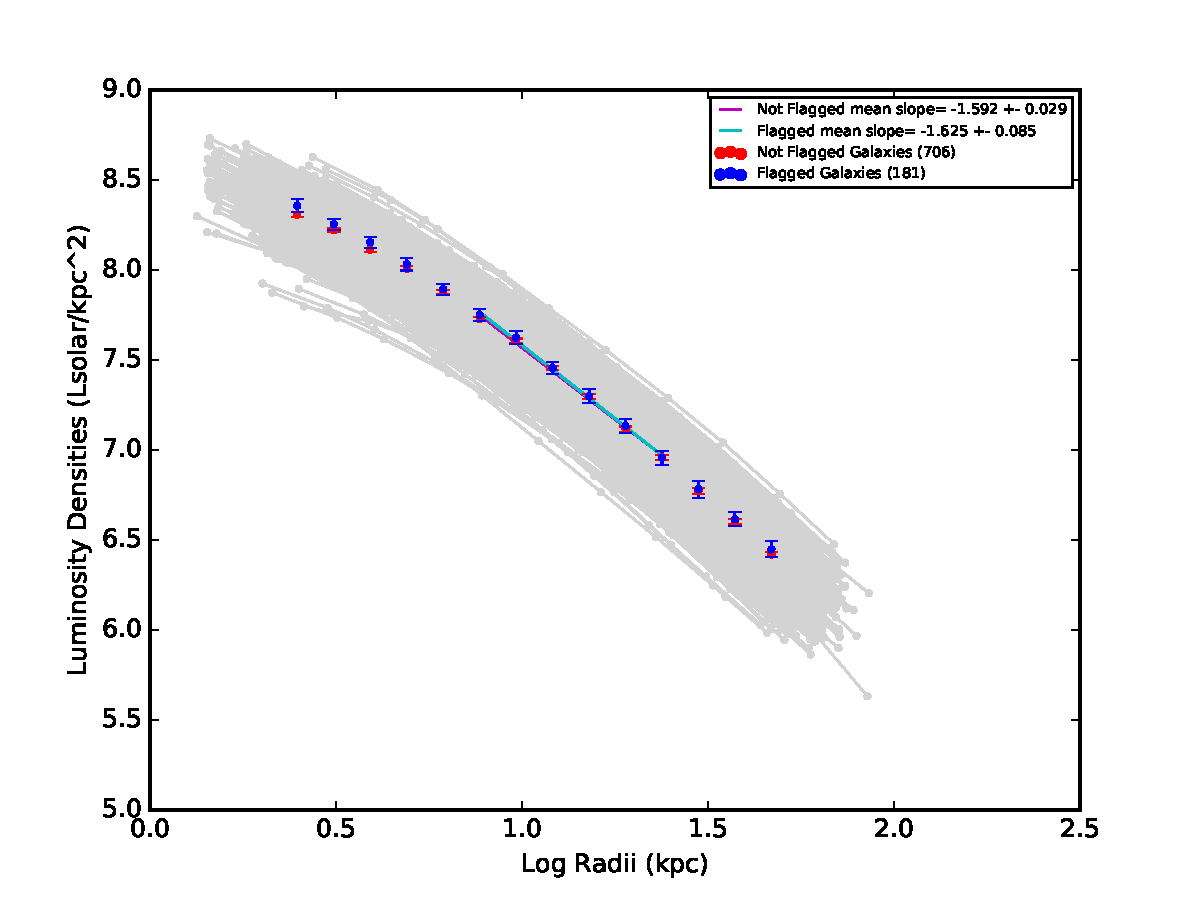
\includegraphics[width=0.5\textwidth]{3meanuplimTF.pdf}}
\hfill
\subfloat[Distribution of alpha\_star slopes\label{subfig:sfigb}]{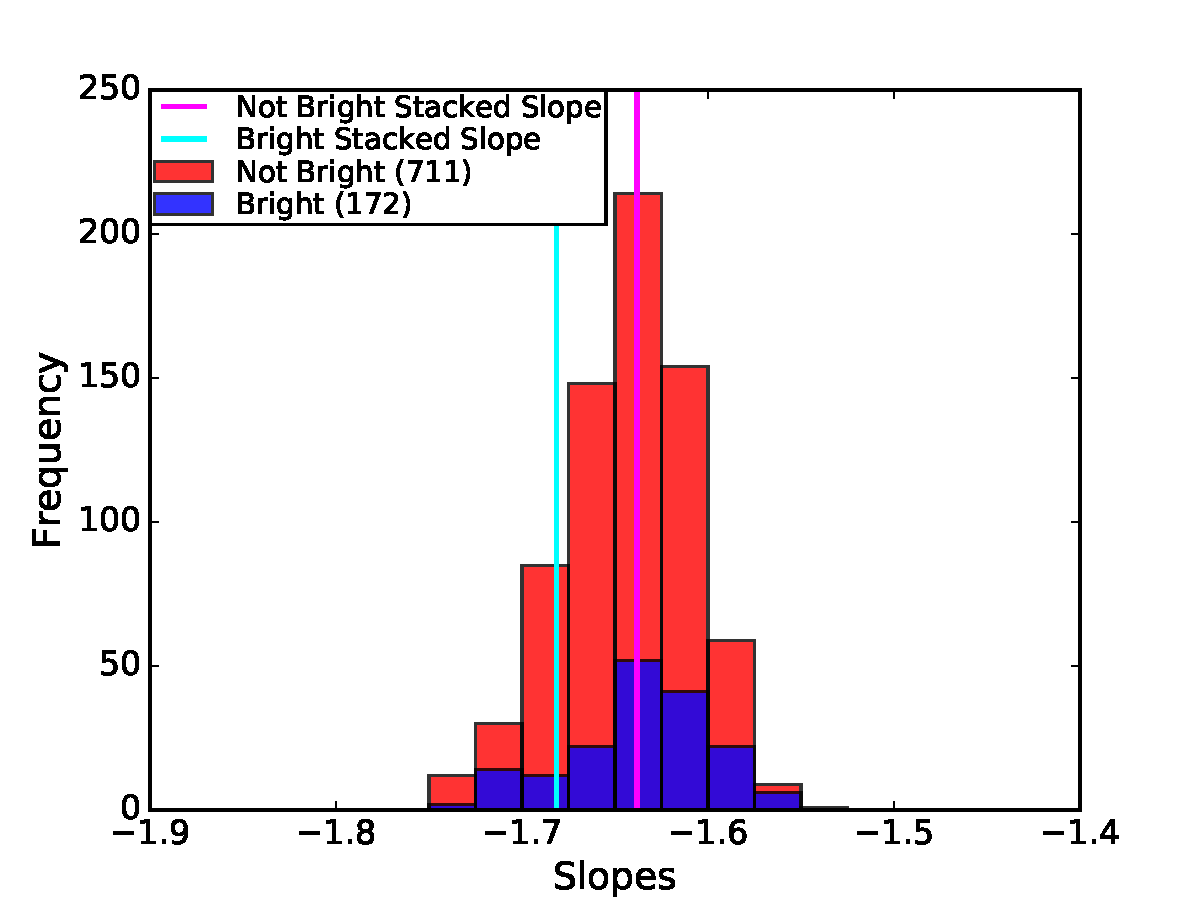
\includegraphics[width=0.5\textwidth]{3meanuplimslopedist.pdf}}
 \caption{Stacked Luminosity Profile for LRG's flagged as Bright Center Objects (blue points), and those not flagged as Bright Center Objects (red points). }
\label{fig:mesh1}
\end{figure}


Varying parts of the stacked profile use distinct galaxies at different redshifts. In order to homogenize our results, so they are all fit to the same physical boundary, we set a uniform outer limit. For our experiment, this outer boundary was exactly 4r1/2 and was applied to both individual galaxies and stacked profiles. As seen in \ref{subfig:sfigb}, by removing the largest apertures from the profile, the mean slope of the flagged and not flagged galaxies are not consistent (within the scatter) with their distributions. This indicates we have removed any parts of the slope at risk of contamination from un-blended sources at the galaxies' envelopes. 

Interestingly, we see that galaxies flagged as bright objects are in agreement with those not flagged. While there appears to be no real difference, we next need to check how these flags alter specific tests we want to accomplish.

\section{SFH and Bright Center Objects}
One test this project is performing is the relationship between the luminosity profile slopes and star formation history (SFH). We use the VESPA code, which fits the spectra of all LRGs in the Sloan Digital Sky Survey's (SDSS) final data release. After matching this catalogue with the LOWZ galaxies, we next separate the LRGs into two different populations, based on whether or not 60\% of the mass of the galaxy is formed in the oldest age bin (between 9.06 and 14 billion years ago). It is important to note that these are all early type galaxies, but we are still distinguishing them by SFH.

\begin{figure}[ht!]
\subfloat[Luminosity Density Profiles\label{subfig:sfig1}]{ 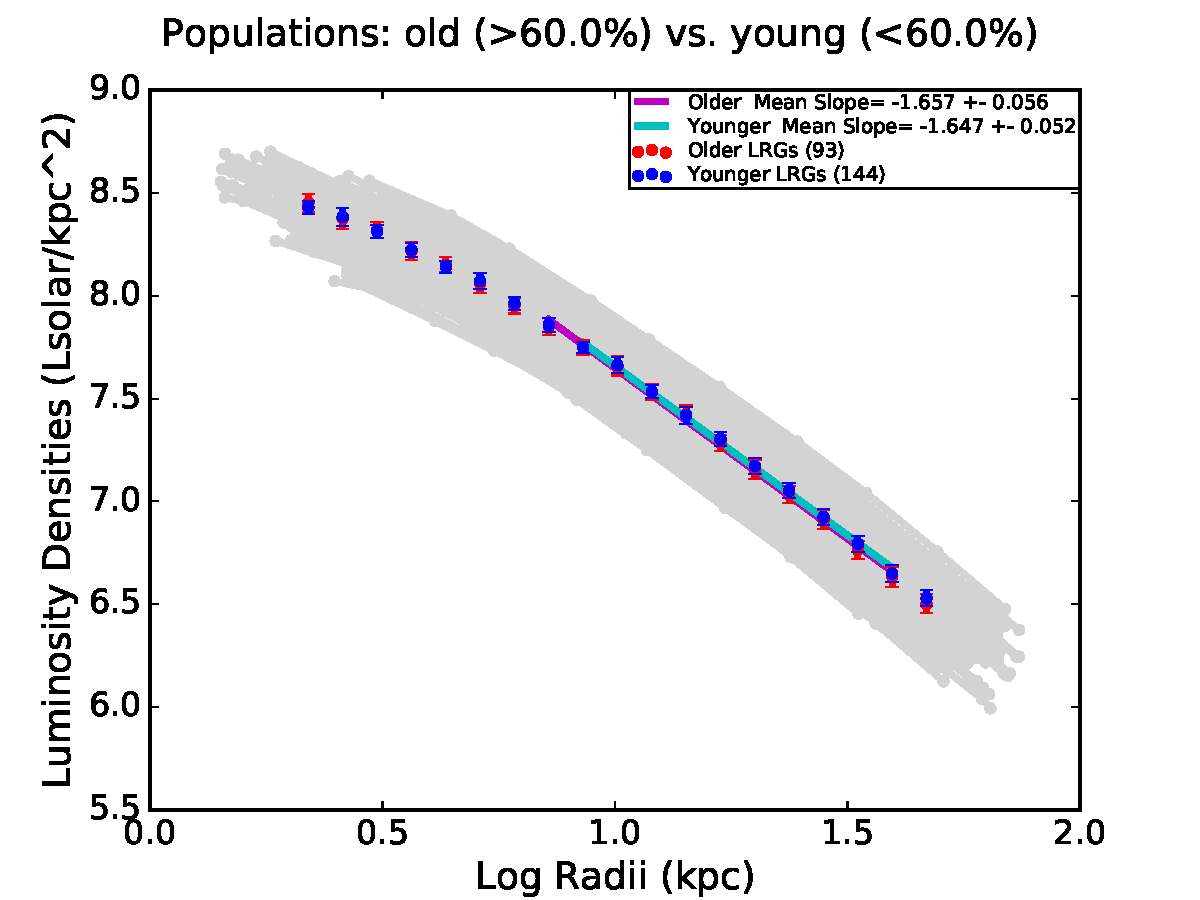
\includegraphics[width=0.5\textwidth]{3oymeanuplimlumage.pdf}}
\hfill
\subfloat[Distribution of alpha\_star slopes\label{subfig:sfig2}]{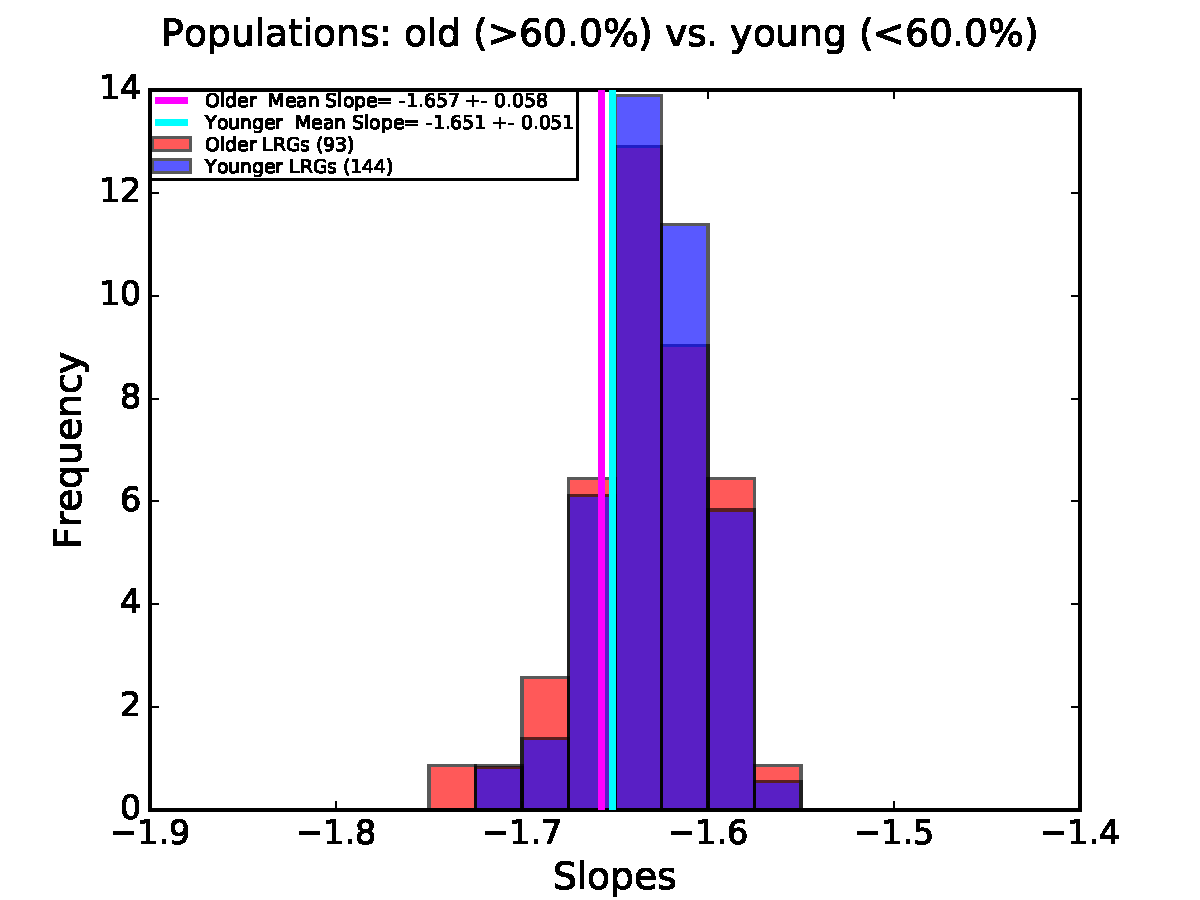
\includegraphics[width=0.5\textwidth]{3oymeanuplimslope_agedist.pdf}}
 \caption{In \ref{subfig:sfig1}, the luminosity profiles of older galaxies (red points) and younger galaxies (blue points). \ref{subfig:sfig2} reveals the distribution of alpha\_star slopes for both populations, as well as the stacked slopes (vertical lines).}
\label{fig:mesh2}
\end{figure}


In Figure 2a, the stacked slopes of older and younger populations of LRGs appear to be roughly the same. Figure 2b reveals that their slope distributions, as well, are very similar.  The stacked slopes coincide with the gaussian distribution within one $\sigma$. However, in order to completely understand our results, we must see how bright center objects affect our graphs.

\begin{figure*}[H!]
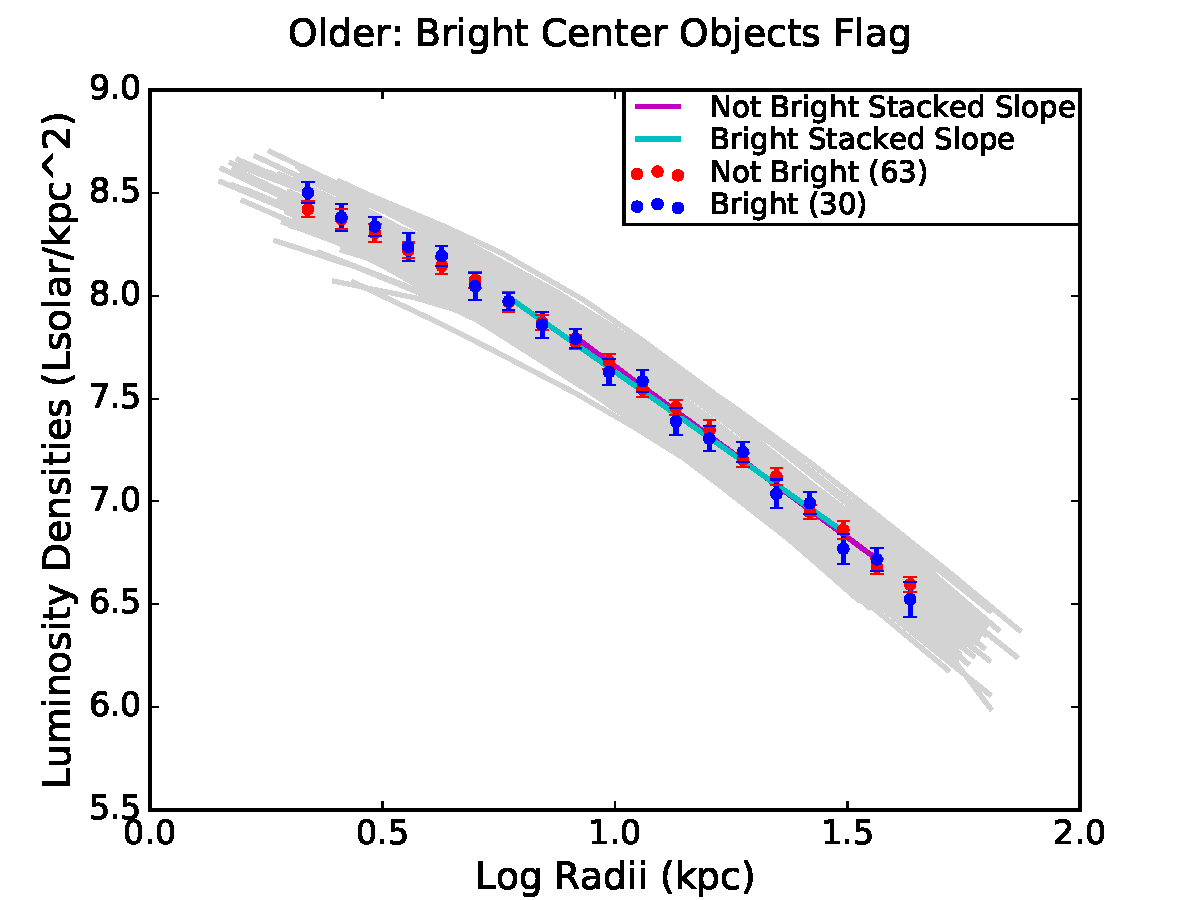
\includegraphics[width=0.5\textwidth,clip]{3oFmeanuplimlumage.pdf}
\label{subfig:sfig3}
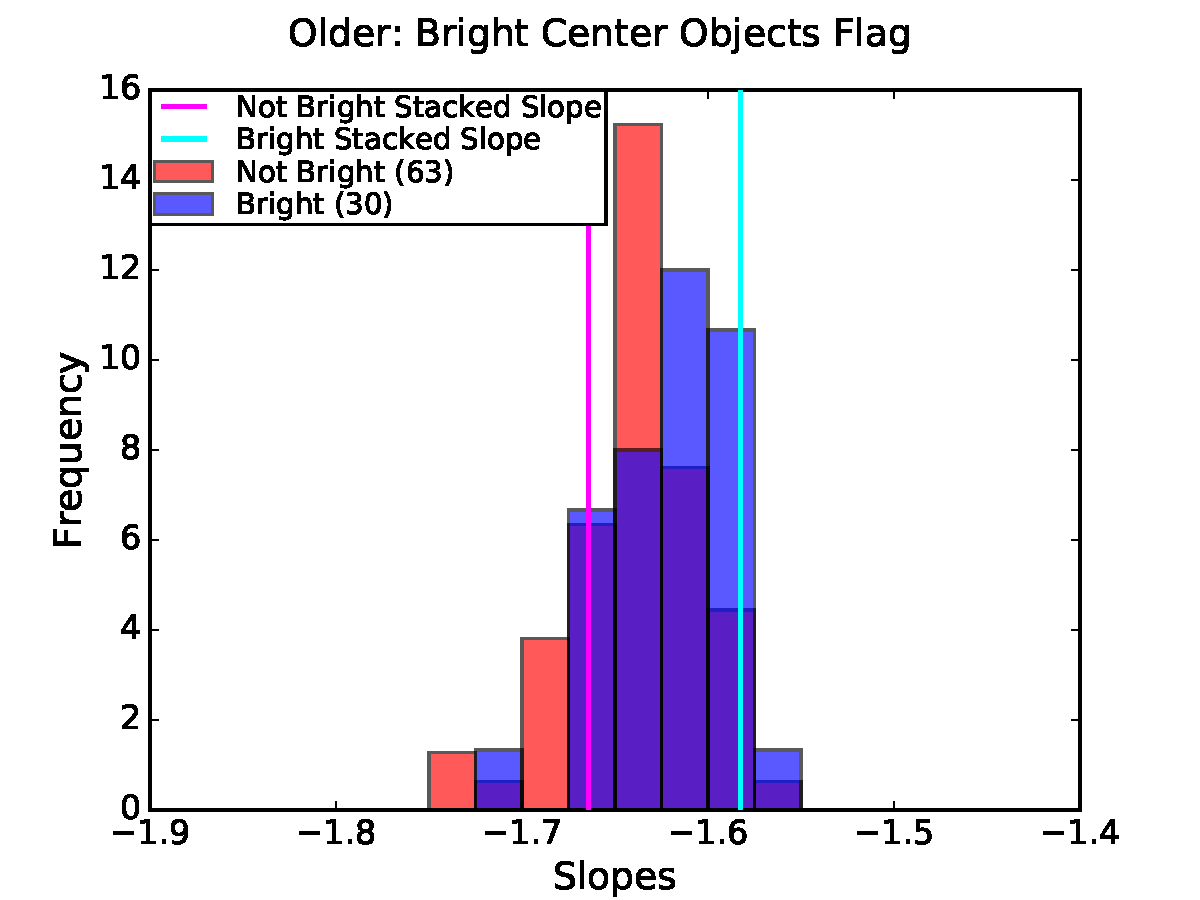
\includegraphics[width=0.5\textwidth,clip]{3oFmeanuplimslope_agedist.pdf}
\label{subfig:sfig4}
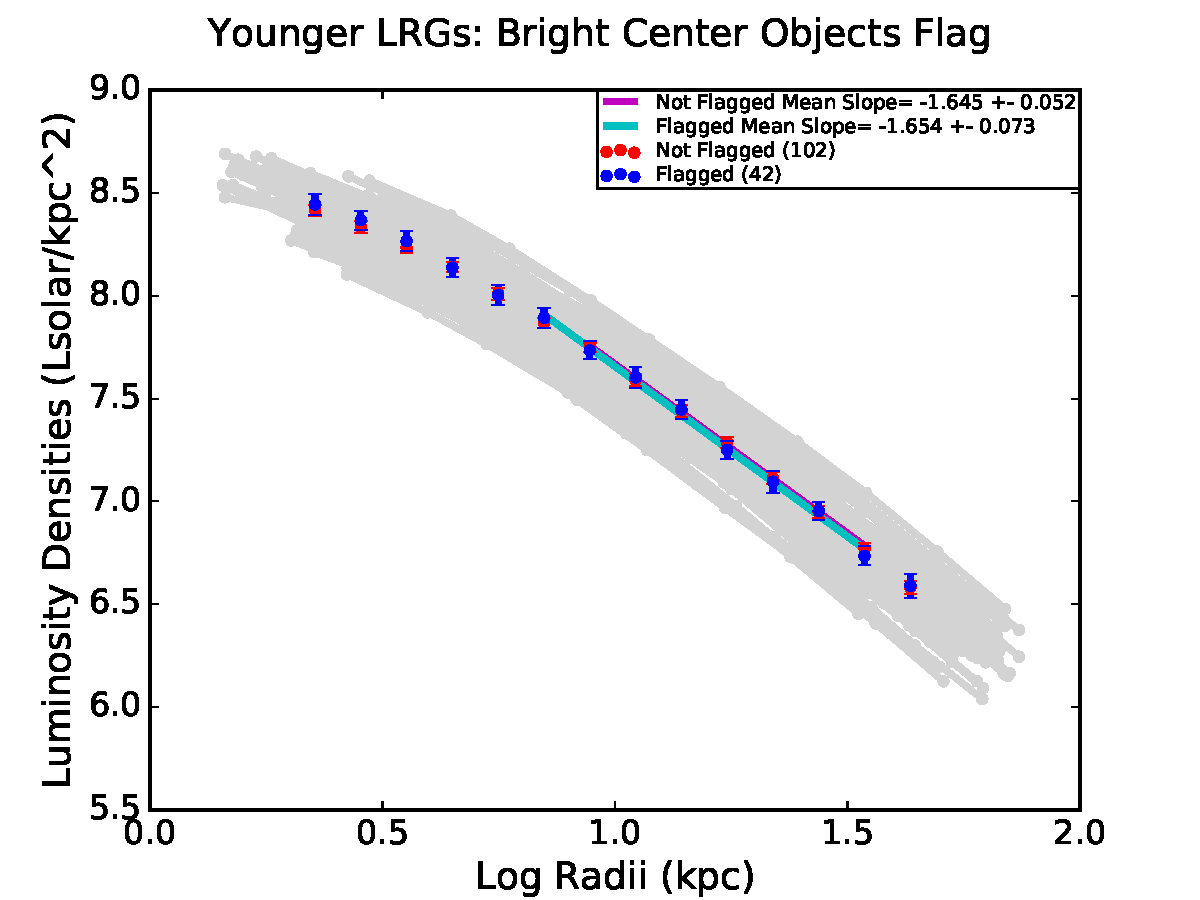
\includegraphics[width=0.5\textwidth,clip]{3yFmeanuplimlumage.pdf}
\label{subfig:sfig5}
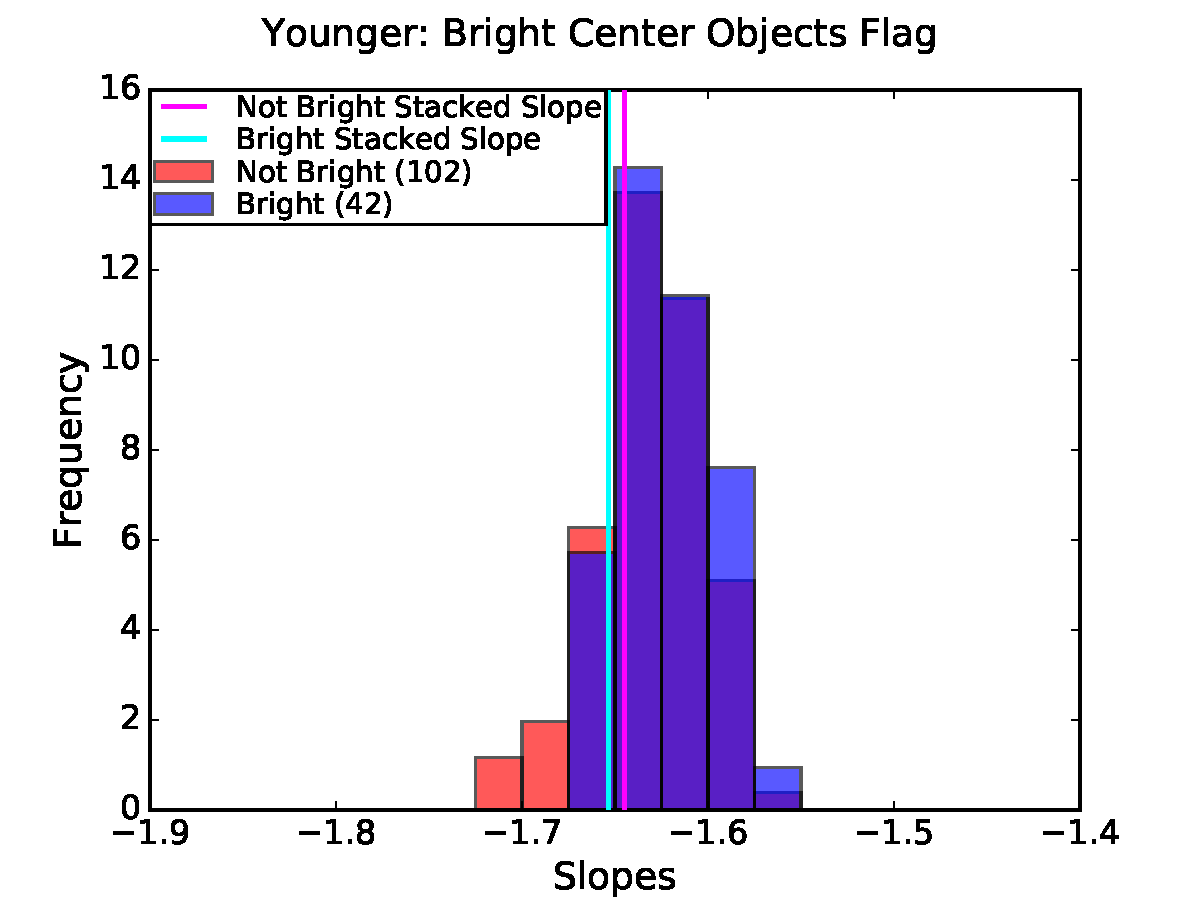
\includegraphics[width=0.5\textwidth,clip]{3yFmeanuplimslope_agedist.pdf}
\label{subfig:sfig6}
\caption{The left\-hand column shows the luminosity profiles of older (upper) and younger (lower) galaxies. Flagged Bright Object Centers are blue points and Not Flagged are red points. The right\-hand column shows the alpha\_star distribution amongst galaxies in each population.}
\label{fig:mesh3}
\end{figure*}

In Figure 3, I separately show the older and younger populations of stars, further split into flagged and not flagged galaxies.

\begin{table}[H]
\centering
\begin{tabular}{ ||c|c|c|| }
\hline
\multicolumn{3}{||c||}{Distribution of Alpha\_Star Slopes}\\
\hline\hline
   & Stacked Slope & Median Slope \\
\hline
Old Galaxies & -1.565 $\pm$ 0.084 &-1.565 \\
\hline
Young Galaxies &-1.597 $\pm$ 0.073 & -1.569\\
\hline
Old and Not Flagged & -1.607 $\pm$ 0.074 & -1.57\\
\hline
Old and Flagged & -1.603 $\pm$ 0.12 & -1.555\\
\hline
Young and Not Flagged & -1.611 $\pm$ 0.066 & -1.569\\
\hline
Young and Flagged & -1.599 $\pm$ 0.119 & -1.57\\
\hline
\end{tabular}
\caption{These stacked and median slopes were calculated from specific population's individual galaxy slope distribution}
\label{table:2}
\end{table}

Table \ref{table:2} compares the alpha\_star slopes of the stacked galaxies with the median of the slope distribution. 

\end{document}